%**********************************************************
\subsection{Task Overview}
One can define and describe briefly how the local system is implemented, making use of threads and processes. As one can see in figure \ref{fig:task_overview}, this system is composed by two processes: the main process and a daemon, used to read the sensors \textit{LDR} and \textit{LampFailureDetector}, \textit{dSensors}. As the \textit{PIR} sensor can be read through the use of an ISR, this sensor stays in the main process. The communication between the daemon and the main process is done via message queue.

\begin{figure}[H]
	\centering
	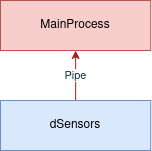
\includegraphics[width=.3\textwidth]{09sw_specification/task_overview}
	\caption{Inter-process Communication between Main Process and Daemon.}
	\label{fig:task_overview}
\end{figure}

\clearpage
One can list the tasks that compose the main process:
\begin{itemize}
	\item \textbf{tCamera:} acquire a camera frame; processes image and search for parking spots; verify the parking spot availability;
%	\item \textbf{tLampControl:} initializes PWM interface; controls the PWM applied to the lamp;
	\item \textbf{tLoraSend:} sends a message to the gateway, using the LoRa module;
	\item \textbf{tLoraRecv:} receives a message from the gateway, using the LoRa module;
	\item \textbf{tRecvSensor:} receives messages sent by the daemon, via message queue, regarding sensors information.
\end{itemize}

%**********************************************************
\subsection{Task Priority}

%**********************************************************
\subsection{Task Synchronization}
Real-time tasks share resources and services, and as such, should be prepared to await for the availability of these resources and services, like logical resources (buffers and data), physical resources, services like directory services, etc. In order to have coordinate access to shared resources and avoid race conditions, the kernel has resources that provide synchronization tools. 

\myparagraph{Condition Variables}

A condition variable is a task synchronization tool that can be used to block (wait) one or more threads, suspending its execution. The blocked threads are awakened when the condition variable is notified. The condition variables used are listed below.

\begin{itemize}
	\item \textbf{condCameraAcquire:} used to notify \textit{tCamera} that a camera sample period has elapsed;
	
%	\item \textbf{condNewPWM:} used to notify \textit{tLampControl} that a new PWM value for the lamp was defined;
	
	\item \textbf{condSend:} used to notify \textit{tLoraSend} that a new message is ready to be sent;
	
	
\end{itemize}

\myparagraph{Mutexes}

A mutex is a locking mechanism that provides mutual exclusion, supporting ownership and other protocols. A mutex is initially created in the unlocked state in which it can be acquired by a task. After being acquired, the mutex moves to the locked state. When the task releases the mutex, it returns to the unlocked state. The mutexes used are listed bellow.

\begin{itemize}
	\item \textbf{mutCamera:} mutex associated with the condition variable \textit{condCameraAcquire} to acquire a camera frame;
		
	\item \textbf{mutSend:} protects the message to be sent in \textit{tLoraSend}, which can be defined in multiple places;
	
	\item \textbf{mutComms:} protects LoRa communication, since it is half-duplex, so one can send or receive at a time; Used in \textit{tLoraSend} and \textit{tLoraRecv};
	
	\item \textbf{mutChangePWM:} protects the modification of PWM when defining a new PWM value for the lamp;
	
	
\end{itemize}

%\myparagraph{Semaphores}

\subsection{Task Communication}
%\myparagraph{Pipes}
%
%Pipe is an inter-process communication tool, that establishes a connection between two processes, such that the standard output from one process becomes the standard input of the other process. Pipe is one-way communication, i.e, we can use a pipe such that one process write to the pipe and the other process reads from the pipe. If a process tries to read before something is written to the pipe, the process is suspended until something is written.
%
%As previously stated, it's used a pipe to communicate between the \textit{dSensors} to the main process. In this way, the main process can know if something was detected by the sensors and provide a response to that.

\myparagraph{Message Queue}

A message queue is a linked list of messages stored within the kernel and identified by a message queue identifier. A message queue will be used to communicate between the main process and the \textit{dSensors}. In that way, the main process is agnostic to the cyclic reading necessary for the sensors \textit{LDR} and \textit{LampFailureDetector}, and is only informed when necessary, thorough the message queue.

%**********************************************************
\subsection{Class Diagrams}
\myparagraph{Class Camera}

In figure \ref{fig:classcamera} is shown the Camera class diagram, that defines a camera object.  For this project the camera is used to detect available parking spots in the lamppost vicinity, so this class defines the functions used to capture (\textit{captureFrame()}) and process (\textit{processFrame}) a camera frame. After the creation of the object, using the constructor \textit{Camera()}, the thread \textit{tCamera()} is executed every time the condition variable \textit{condCameraAcquire} is signaled, that happens every 2 minutes.

%This class defines all the functions that implicate the use of the camera device.

\begin{figure}[H]
	\centering
	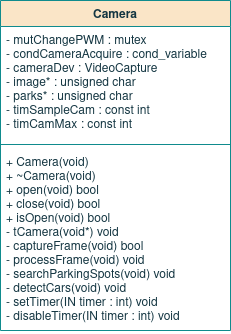
\includegraphics[width=.5\textwidth]{09sw_specification/classcamera}
	\caption{Class Diagram: Camera.}
	\label{fig:classcamera}
\end{figure}

\myparagraph{Class Lamp}

In figure \ref{fig:classlamp} is shown the Lamp class diagram, which defines a Lamp object. After creating the object, using the constructor \textit{Lamp()}, one can interact with it by changing the brightness, through the method \textit{setBrightness(lux)}, where \textit{lux} is a value from 0, lamp OFF, to 100, lamp at maximum brightness. Internally, this class uses a mutex, \textit{mutChangePWM} to protect the PWM value when using \textit{setBrightness} method. 

\begin{figure}[H]
	\centering
	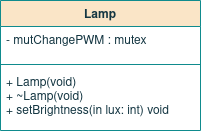
\includegraphics[width=.5\textwidth]{09sw_specification/classlamp}
	\caption{Class Diagram: Lamp.}
	\label{fig:classlamp}
\end{figure}

\myparagraph{Class Communications}

In figure \ref{fig:classcomm} is shown the Communications class diagram. This class defines an object Communication capable of establishing a LoRa communication with the gateway, through the use of the constructor \textit{Communication()}, and send messages through the use of \textit{Send(msg)}. It's used a vector of messages \textit{queued\_msgs} to store the message that's in the waiting list to be sent, in order to avoid the loss of a communication. To exchange messages are used two threads, \textit{tLoraSend} to send, and \textit{tLoraRecv} to receive, which makes use of task synchronization tools to ensure that sending and receiving don't occur at the same time, since the LoRa module in use is Half-Duplex.

\begin{figure}[H]
	\centering
	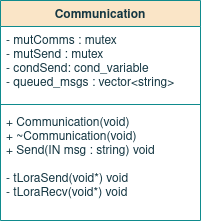
\includegraphics[width=.5\textwidth]{09sw_specification/classcomms}
	\caption{Class Diagram: Communications.}
	\label{fig:classcomm}
\end{figure}

\myparagraph{Class PIR}

In figure \ref{fig:classpir} is shown the PIR class, that defines the functions to interact with the PIR sensor. When movement is detected in the surrounding area of the lamppost, the sensor puts the high digital value in its output, triggering the interrupt service routine \textit{PirIsr}.

\begin{figure}[H]
	\centering
	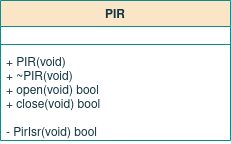
\includegraphics[width=.5\textwidth]{09sw_specification/classpir}
	\caption{Class Diagram: PIR.}
	\label{fig:classpir}
\end{figure}

\myparagraph{Class LDR}

In figure \ref{fig:classldr} is shown the LDR class, that defines the functions to interact with the LDR sensor, using its device driver. As the ambient light is read each 10 minutes in the function \textit{LdrIsr}, one needs to define a timer to trigger this function. The last read luminance is stored in the variable \textit{oldLightCon} and is obtained using the function \textit{getLux}.

\begin{figure}[H]
	\centering
	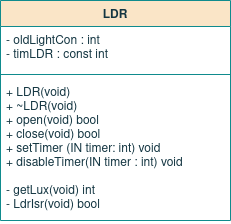
\includegraphics[width=.5\textwidth]{09sw_specification/classldr}
	\caption{Class Diagram: LDR.}
	\label{fig:classldr}
\end{figure}

\myparagraph{Class FailureDetector}

In figure \ref{fig:classfail} is shown the Failure Detector class. After creating an instance of this class, using the contructor \textit{FailureDetector}, the function \textit{failureDetectIsr} will be triggered each time the failure detector senses the lamp failure. 

\begin{figure}[H]
	\centering
	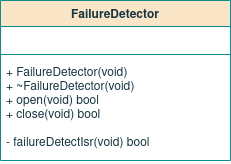
\includegraphics[width=.5\textwidth]{09sw_specification/classfail}
	\caption{Class Diagram: FailureDetector.}
	\label{fig:classfail}
\end{figure}

%**********************************************************
\subsection{Flowcharts}
%\clearpage
\myparagraph{tCamera}

The task tCamera is responsible for acquire a frame from the Raspberry Pi Camera and to process it. It must analyze the returned frame, in order to detect empty parking spots. This thread uses the mutex \textit{mutCamera} to protect the condition variable \textit{condCameraAcquire}, that synchronizes the camera frame acquisition with the timer that defines the camera frame acquisition period, \textit{timSampleCam}.

Firstly, this thread initializes the camera device, sets the timer \textit{timSampleCam}, locks the mutex \textit{mutCamera} and goes to sleep mode, waiting for the conditon variable \textit{condCameraAcquire} to be signaled. This happens when a \textit{timSampleCam} period has elapsed and the thread wakes up. Now, one can capture a camera frame in order to process it, unlocking the mutex \textit{mutCamera}. A timer, \textit{timCamMax}, is setted to report the error if the image is taking too much time to being processed.

In the image processing part of the thread, if there aren't parking spots coordinates stored, then it is necessary to search for parking spots. After that, one can detect cars using the pre-trained model and the function \textit{detectCars} that detects cars in the image. If the coordinates of a detected car matches the coordinates of the parking spot, then one can assume that the parking spot is occupied. If the parking spot status has changed, then it is necessary to send this to the remote system, using the LoRa communication module.

\myparagraph{tRecvSensors}

This task, presented in figure \ref{fig:flow_trecv_sensors}, is responsible for receiving messages sent by the sensors daemon, through a message queue.

When the message queue is not empty, this task reads a message from the message queue and parses it, in order to find out which sensor was triggered and what action this system should take. For that, a list of commands may be defined:
\begin{itemize}
%	\item Lamp Max: the lamp brightness must be at its maximum (PWM=100);
	\item Lamp Min: the lamp must be at minimum bright level (PWM = \textit{MIN\_BRIGHT\_PWM});
	\item Lamp OFF: the lamp must be OFF (PWM=0);
	\item Lamp Fail: the lamp must be OFF, since there was a failure detected on the lamp.
\end{itemize}

\begin{figure}[H]
	\centering			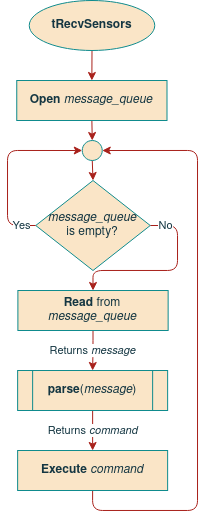
\includegraphics[width=.4\textwidth]{09sw_specification/trecvsensors}
	\caption{Main Process Flowchart: tRecvSensors.}
	\label{fig:flow_trecv_sensors}
\end{figure}

%**********************************************************
\clearpage
\myparagraph{Class Lamp Constructor and Destroyer}

This functions, presented in figure \ref{fig:flow_lampconstruct}, are responsible for initializing and destroying a Lamp object. First, in the constructor, which is the left side function, the PWM peripheral is initialized, then the mutex that is used to protect the change of PWM is also initialized. On the destroyer side, the opposite is done, by the terminating the PWM generation.

\begin{figure}[H]
	\centering	
	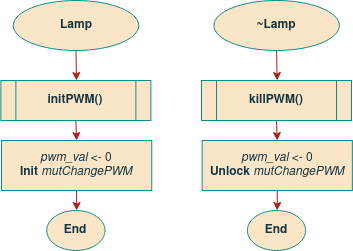
\includegraphics[width=.7\textwidth]{09sw_specification/lampconstruct}
	\caption{Class Lamp Flowchart: Constructor and Destroyer.}
	\label{fig:flow_lampconstruct}
\end{figure}

\myparagraph{setBrightness}

This function, presented in figure \ref{fig:flow_setbrightness}, is responsible for changing the PWM associated with the lamp, which is directly related to its brightness. Through \textit{setPWM(lux)} one can change the current lamp PWM to \textit{lux} value, being this an integer between 0 to 100. When the PWM is maximum, a timer is started that defines how much time the lamp is ON, \textit{LAMP\_ON\_TIMEOUT} in seconds, if there isn't another call of this function.

\begin{figure}[H]
	\centering	
	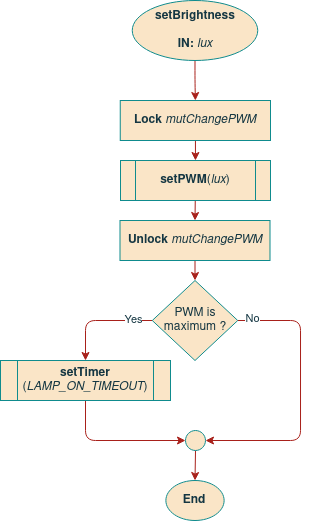
\includegraphics[width=.6\textwidth]{09sw_specification/lampsetbrightness}
	\caption{Class Lamp Flowchart: setBrightness.}
	\label{fig:flow_setbrightness}
\end{figure}


%**********************************************************
\clearpage
\myparagraph{Class Communication Constructor and Destroyer}

This functions, presented in figure \ref{fig:flow_commconstruct}, are responsible for initializing and destroying a Communication object. On the left side, the constructor, starts by initializing the LoRa communication, defining the frequency in which the device choosen previously operates, which is 433~MHz. Then the messages vector is cleared, the mutexes are initialized and the two threads responsible for the exchange of messages between the local system and the gateway are created. In the destroyer side, one has the opposite, where the LoRa communication is disabled and the threads are terminated.

\begin{figure}[H]
	\centering			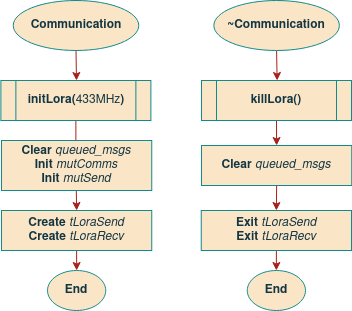
\includegraphics[width=.7\textwidth]{09sw_specification/commsconstruct}
	\caption{Class Communication Flowchart: Constructor and Destroyer.}
	\label{fig:flow_commconstruct}
\end{figure}

\myparagraph{tLoraSend}

This task is responsible for sending queued messages to the gateway, using LoRa communication. A conditional variable is used to wake this thread when there is a new message available to be sent.

When the vector \textit{queued\_msgs} is empty, then the task goes to sleep, waiting for the condition variable \textit{condSend} to notify this task. This happens when a new message is inserted into the messages vector, using \textit{Send(msg)} function, that will be later presented. After this, the mutex \textit{mutComms} is used to protect the communication, which due to the selected LoRa module is half-duplex, meaning that at a given moment, the device can be receiving or sending, not at the same time. Then, a message is popped from the messages vector, and sent to the gateway using the function \textit{LoraSend}. This continues to happen until the \textit{queued\_msgs} vector gets empty.

The flowchart for this task is presented in figure \ref{fig:flow_tlorasend}

\begin{figure}[H]
	\centering		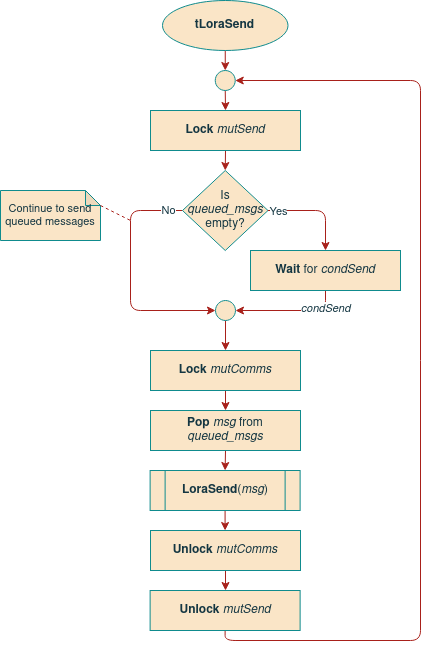
\includegraphics[width=.85\textwidth]{09sw_specification/commstlorasend}
	\caption{Class Communication Flowchart: tLoraSend.}
	\label{fig:flow_tlorasend}
\end{figure}


\myparagraph{tLoraRecv}

This task is responsible for receiving messages from the gateway, using LoRa communication.

When a message is received, using \textit{LoraReceive}, this is parsed and later, the respective command will be executed.

The flowchart for this task is presented in figure \ref{fig:flow_tlorarecv}

\begin{figure}[H]
	\centering		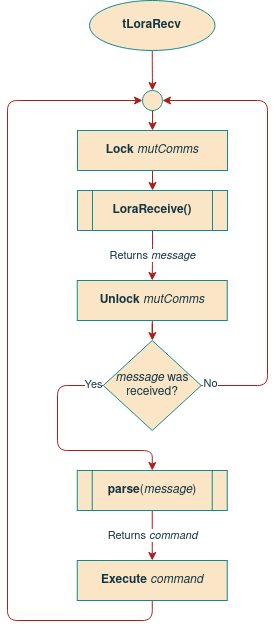
\includegraphics[width=.55\textwidth]{09sw_specification/commstlorarecv}
	\caption{Class Communication Flowchart: tLoraRecv.}
	\label{fig:flow_tlorarecv}
\end{figure}

\myparagraph{Send}

This function, presented in figure \ref{fig:flow_send}, is responsible for adding a new message, \textit{msg}, to the \textit{queued\_msgs} vector, and signal the condition variable \textit{condSend}, for the task \textit{tLoraSend} to send the message.

\begin{figure}[H]
	\centering	
	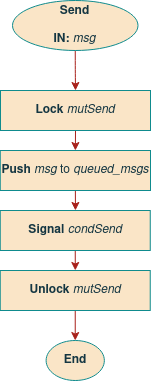
\includegraphics[width=.3\textwidth]{09sw_specification/commssend}
	\caption{Class Communication Flowchart: Send.}
	\label{fig:flow_send}
\end{figure}


% FLOWCHARTS SENSORS

\myparagraph{PirIsr}
The PIR sensor uses the GPIO of the Raspberry Pi in order to inform the system if there's movement in the surrounding area. In the afirmative case, it puts the high digital value on its output, and this can be used to generate an interrupt service routine, triggered on the rising edge of the output signal of the sensor. When this routine is executed, it locks the mutex \textit{mutChangePWM} and assign the \textit{PWM\_val} its maximum value, 100 \%, unlocking the mutex. Now, one needs to send the PWM value to the remote system through the LoRa communications, in order to be updated in the remote system. In the figure \ref{fig:pir_isr}, is represented the flowchart of the PirIsr function.

\begin{figure}[H]
	\centering
	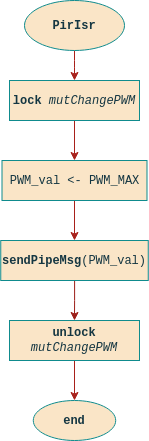
\includegraphics[width=.2\textwidth]{09sw_specification/pir_isr}
	\caption{PirIsr flowchart.}
	\label{fig:pir_isr}
\end{figure}

\myparagraph{LdrIsr}
The ambient light sensor, LDR, is used to determine when is time to turn on the lights, that is, when is night time and interfaces with the Raspberry Pi through I2C protocol communication. As the sun set or the sun rise is a relatively long time process, there's no need to keep checking the sensor output value all the time, so one can define a period to get the sensor value, \textit{LDR\_TIM}, that can be 10 minutes. In figure \ref{fig:ldr_isr} is shown the LDR sensor interrupt service routine, triggered by the timer overflow. When the timer period elapses, the illuminance value is calculated by the sensor. If this value is lower than the threshold value defined as good luminosity illuminance, GOOD\_LIGHT\_LUX, then the auxiliary variable, \textit{lightCon} is setted to high. In the next step, if the \textit{oldLightCon} variable (stores the last ambient light condition) is not equal to the auxiliary variable, then it is needed to change the \textit{oldLightCon} variable and send message to the process that controls the lamp PWM, through message queue. 

\begin{figure}[H]
	\centering
	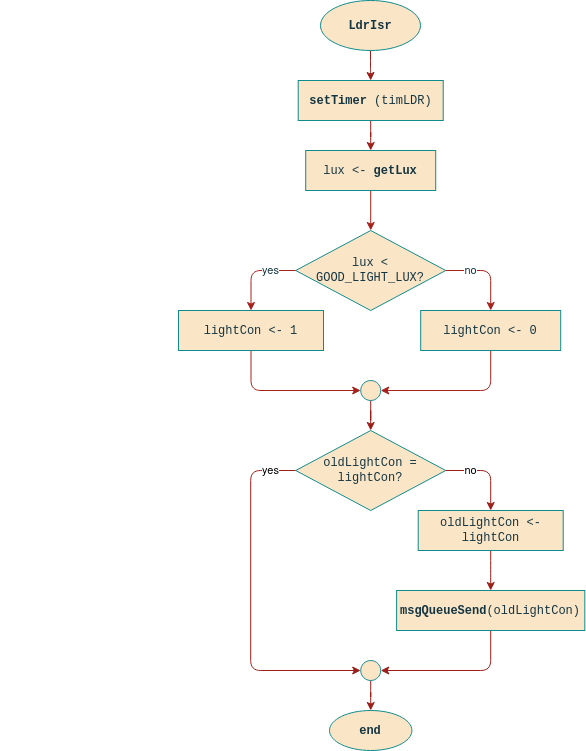
\includegraphics[width=.4\textwidth]{09sw_specification/ldr_isr}
	\caption{LdrIsr flowchart.}
	\label{fig:ldr_isr}
\end{figure}

\myparagraph{FailureDetectIsr}
In figure \ref{fig:fail_isr} is represented the FailureDetectIsr flowchart. Similarly to the PIR sensor, this routine is triggered on the rising edge of the output signal of the sensor. When the Failure detector detects that the lamp is broken, it puts the high digital value in its output, triggering this function. In this routine, the PWM is setted to 0 \% and are sent two messages through message queue: one to inform the process, that controls the lamp, to change the PWM value in the channel; and the other to notify the remote system that the lamp is broken, in order to update this status on the database.

\begin{figure}[H]
	\centering
	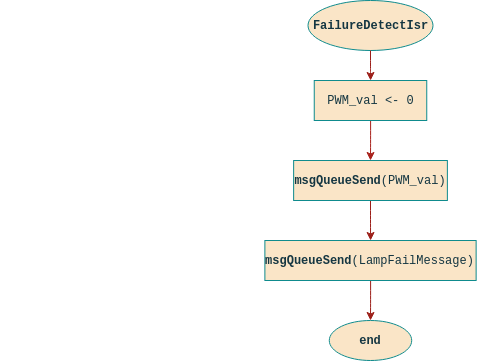
\includegraphics[width=.3\textwidth]{09sw_specification/fail_isr}
	\caption{FailureDetectIsr flowchart.}
	\label{fig:fail_isr}
\end{figure}

%**********************************************************
\subsection{Start-up Process}

%**********************************************************
\subsection{Shutdown Process}

%\myparagraph{tLampControl}
% uses: mutChangePWM; condNewPWM; pwm_val
% pwm_val is used in: PIR_sensor, CommandCb, LDR
% must define: MIN_BRIGHT_PWM; LAMP_ON_TIMEOUT
%This task is responsible for initializing and controlling the PWM peripheral used to control the lamp brightness. A mutex \textit{mutChangePWM} is used to protect the process of defining a new PWM value. 
%
%After initializing the PWM, this task goes to sleep, waiting for the condition variable \textit{condNewPWM} to notify this task. This happens when a new PWM value is defined into the variable \textit{pwm\_val}, in \textit{dReadSensors} or in a received command. Then, the lamp PWM is changed to the new value. 
%
%The lamp may have various levels of luminosity: for the lamp to be OFF, is applied PWM~=~0; for the lamp to be at a predefined minimum bright level, is applied PWM~=~\textit{MIN\_BRIGHT\_PWM}; for the lamp to be at maximum bright, this is, when the lamp must be ON, is applied PWM~=~100. So, since the lamp must stay ON a minimum amount of time out of a motion is detected or out of a request from the remote system to be ON, one needs to check if the new PWM is the maximum value. If so, that means that the lamp should continue with that PWM for a predefined time, defined by \textit{LAMP\_ON\_TIMEOUT}, in seconds.
